\documentclass{beamer}
\usepackage[utf8]{inputenc}
\usepackage[english]{babel}
\setbeamersize{text margin left=10pt, text margin right=10pt} %new code
\usepackage{graphicx}
\usepackage{float}
\usepackage{subcaption}

\usepackage{animate}
\usepackage{movie15}
\usepackage{breqn, bm}
\usepackage{tcolorbox, amsmath}
\usepackage{subcaption, minted}
\newcommand{\mysetminus}{\mathbin{\fgebackslash}}

\definecolor{notgreen}{RGB}{255,127,0}
\definecolor{green}{RGB}{49,150,3}
\setbeamerfont{headline}{size=\small}


%----------------------------------------------------------------------------------------
%	 Package
%----------------------------------------------------------------------------------------
\usepackage{color}
\usepackage{url}
\usepackage{minted}		% listing code
\beamertemplatenavigationsymbolsempty

\definecolor{cadmiumred}{rgb}{0.8, 0.8, 0.8}

%----------------------------------------------------------------------------------------
%	 Presentation settings
%----------------------------------------------------------------------------------------

\usetheme{CambridgeUS}
\usecolortheme{beaver}


\setbeamertemplate{itemize items}[triangle] 
\setbeamertemplate{enumerate items}[default]
 
\title[Neural Nets for Texts]{
	Text Analysis Course \\ 
	\vspace{1cm}
	\textbf{\textcolor{black}{Neural Nets for Texts}}}

\author{Ashuha Arseniy}
\institute[MIPT]{
	Moscow Institute of Physics and Technology\\
	Department of Innovation and High Technology
	
	
	\medskip
	
	\href{mailto:ars.ashuha@gmail.com}{\nolinkurl{ars.ashuha@gmail.com}}}

\date{\today}

\newcommand{\Expect}{\mathsf{E}}
\newcommand{\MExpect}{\mathsf{M}}
\newcommand{\cov}{\mathsf{cov}}


\begin{document}
\begin{frame}
	\titlepage 
\end{frame}

\section*{Introduction}
	\subsection*{Text Classification}
	\begin{frame}
	 The task is to assign a document $\bm{x}$ to one or more classes or categories $\bm{y}$
	 \vspace{1ex}
			\begin{itemize}
				\item Linear Models ($\hat{y}$ -- scores vector)
					 \begin{columns}[onlytextwidth]
					 	\begin{column}{0.7\textwidth}
					 		\centering
					 		{\small$$\hat{y}(\bm{x}; W, \bm{b}) = W\bm{x} + \bm{b}$$}
						 	\vspace{0.05cm}
					 	\end{column}
					 	\begin{column}{0.25\textwidth}
					 		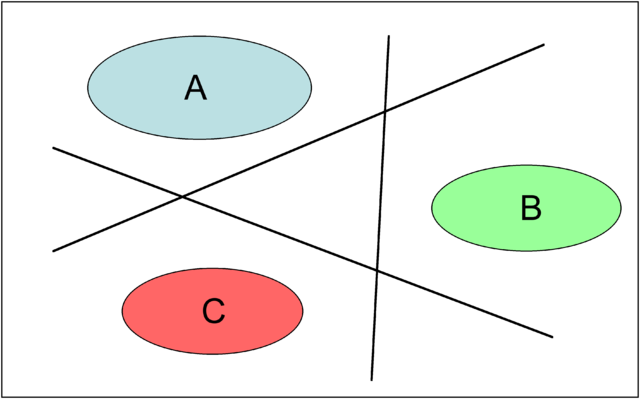
\includegraphics[scale=0.6]{img/multiclass_svm.png}
					 	\end{column}
					\end{columns}
					
					
				\vspace{-0.1cm}
				\item Reduce Dimensions and Ensembles
					 \begin{columns}[onlytextwidth]
					 	\begin{column}{0.65\textwidth}
					 		\centering
					 					
		 					{\small$$
		 					\hat{y}(\bm{x}; T)  = \frac{1}{|T|}\sum_i T_i(low\_dim(\bm{x}))
		 					$$}
		 				
					 	\end{column}
					 	\begin{column}{0.35\textwidth}
					 		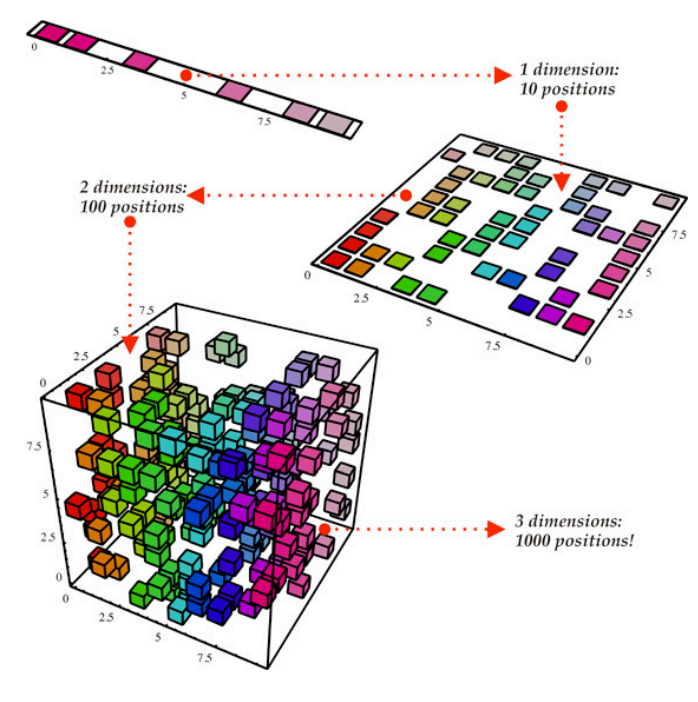
\includegraphics[scale=0.08]{img/reduce_dim.png}
					 		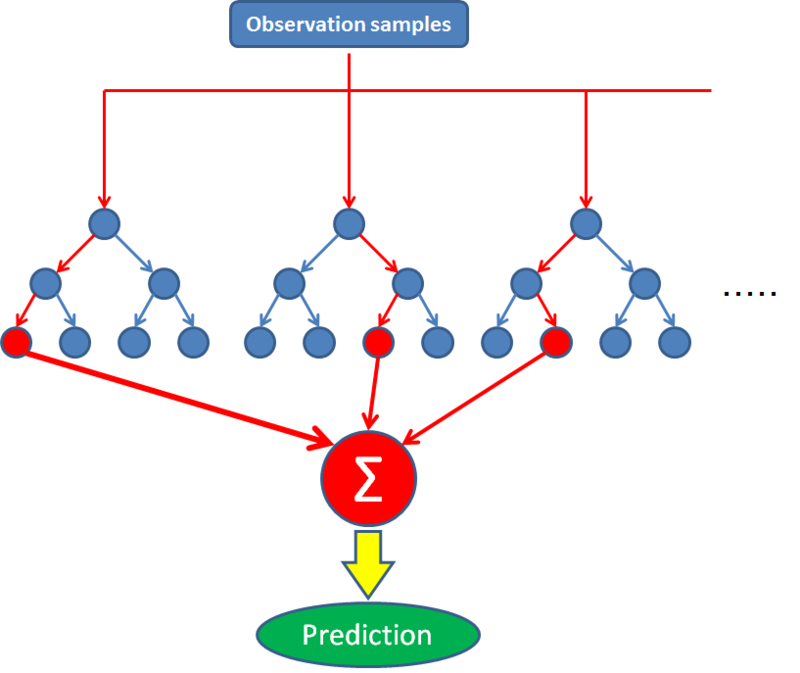
\includegraphics[scale=0.09]{img/random_forest.png}					 	
					 	\end{column}
					\end{columns}
				
				\vspace{-0.1cm}
				\item Neural Nets
					 \begin{columns}[onlytextwidth]
								 	\begin{column}{0.75\textwidth}
								 		\centering
								 		
										{\small$$
										\hat{y}(\bm{x}; W, \bm{b}) = W^2\sigma(W^1\bm{x} + \bm{b}^1 ) + \bm{b}^2
										$$}
										\vspace{0.1cm}
				
								 	\end{column}
								 	\begin{column}{0.25\textwidth}
								 		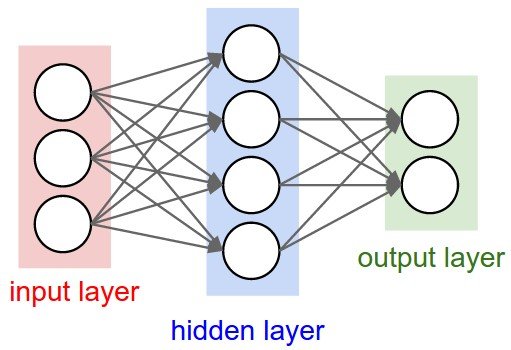
\includegraphics[scale=0.14]{img/two_layer_nn}	 	
								 	\end{column}
					 \end{columns}
				

			\end{itemize}
			
			\vspace{-0.3cm}
			\begin{tcolorbox}[colback=gray!0, colframe=red!90]
				\centering {\small How to 1) take into account the words range 2) make features} automatic
			\end{tcolorbox}
	\end{frame}

	\subsection*{Sequential Inputs}
	\begin{frame}			
			\begin{figure}
				\begin{subfigure}{.49\textwidth}
					\centering				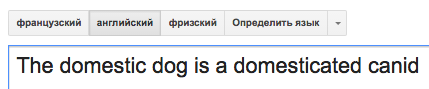
\includegraphics[scale=0.35]{img/transl1} 
		
					\hspace{0.60cm}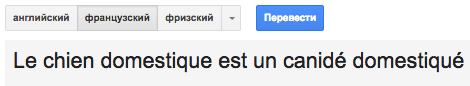
\includegraphics[scale=0.35]{img/transl2}
					\caption{Machine Translation }
				\end{subfigure}
				\begin{subfigure}{.49\textwidth}
					\vspace{0.2cm}
					\centering 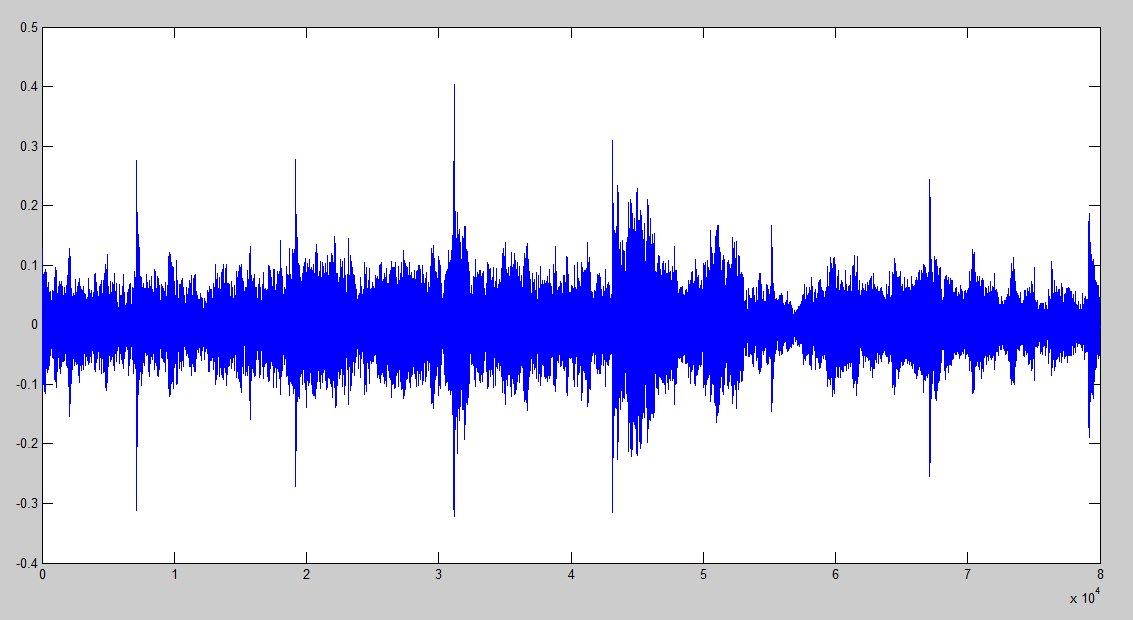
\includegraphics[scale=0.15]{img/audio} 
					\caption{Speech Recognition}
				\end{subfigure}
				
				\vspace{0.2cm}
				
				\begin{subfigure}{.49\textwidth}
					\vspace{1.5cm}
					\centering  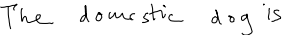
\includegraphics[scale=0.7]{img/hand_write} 
					\caption{Handwritten Generation }
				\end{subfigure}
				\begin{subfigure}{.49\textwidth}
					\centering 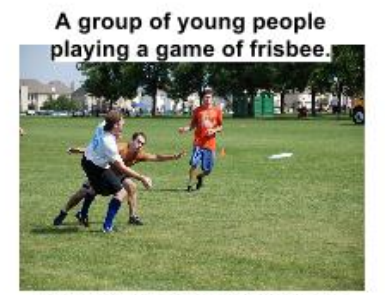
\includegraphics[scale=0.2]{img/image_ann} 
					\caption{Image Annotation}
				\end{subfigure}
			\end{figure}
			
			
	\end{frame}
	
	\subsection*{Rid the Bag of Words, Embeding Idea}
	\begin{frame}
		\begin{itemize}
			\item Let's back to Text Classification
			\item Bag of Words is really bad idea, we need to save \textcolor{red}{sequence structure}
			\item Map each word to vector (Embedding)
			
		 \vspace{0.4cm}
		 \begin{columns}[onlytextwidth]
		 	\begin{column}{0.4\textwidth}
		 		\centering 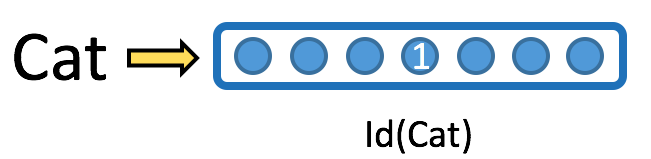
\includegraphics[scale=0.2]{img/one_hot} 
				\centering \hspace{1cm} One Hot Encoding
		 	\end{column}
		 	
			 \begin{column}{0.5\textwidth}
			 	\centering 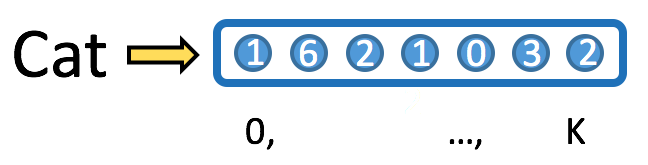
\includegraphics[scale=0.2]{img/w2v} 
			 	
				\centering Word2Vec
			 \end{column}			 
		\end{columns}
		
		\vspace{0.4cm}
		\item Represent Text as a vector sequence
		
		\begin{center}
			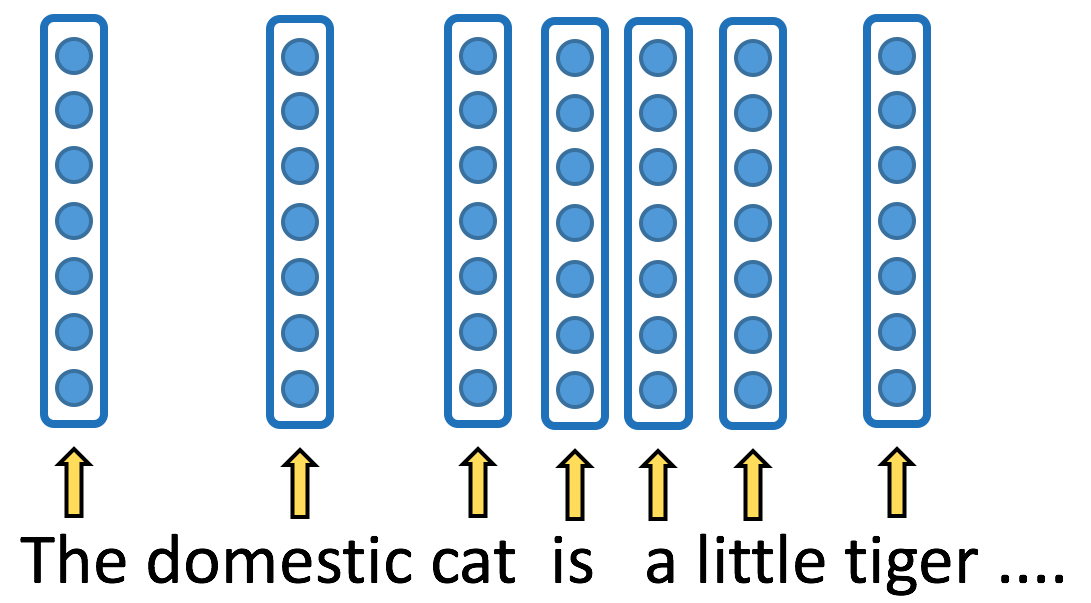
\includegraphics[scale=0.16]{img/text_repr} 
		\end{center} 
		
	  \end{itemize}
		
	\end{frame}
	
	\section{Recurrent Neural Nets}
	\subsection*{Main Idea}
	\begin{frame}
		\begin{center}
			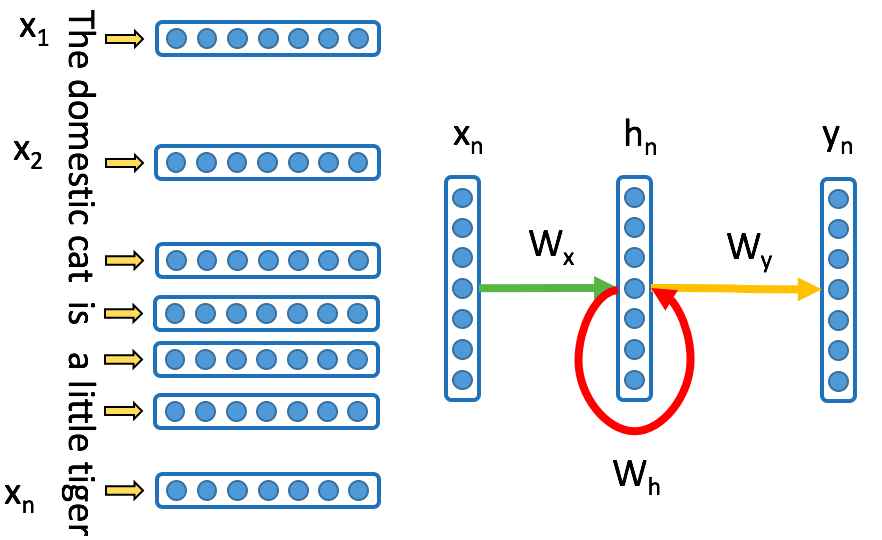
\includegraphics[scale=0.35]{img/recurrent_nn}
		\end{center}
		\vspace{-0.5cm}
		$$h_n = \textcolor{green}{W_x} x_n + \textcolor{red}{W_h}\sigma(h_{n-1})$$
		$$y_n = \sigma(\textcolor{notgreen}{W_y}  h_n)$$
		
	\end{frame}
	
	\subsection*{How to Train Linear Models}
	\begin{frame}
		
			{\small$$\hat{y}(\bm{x}; W, \bm{b}) = W\bm{x} + \bm{b}$$}
			\begin{itemize}
				\item Introduce and optimize loss function 
					$$L(X, y, W, b) = \sum_i ||\hat{y}(\bm{x}_i; W, \bm{b}) - y_i||^2 \rightarrow \min_{W, b}$$
				\item Evaluate Gradients
					The gradient is matrix/vector construct from  
					$$\frac{\partial L}{\partial W_{ij}} = ... ~~~~ \frac{\partial L}{\partial b_{i }} = ...  $$
				\item Run you favourite optimization Method
			\end{itemize}
	\end{frame}
	
	
	\subsection*{How to Train Neural Nets}
	
		\begin{frame}
			
				{\small
					$$
					\hat{y}(\bm{x}; W, \bm{b}) = W^2\sigma(W^1\bm{x} + \bm{b}^1 ) + \bm{b}^2
					$$
					\begin{align*}
						f^1 (x)  = \sigma(W^1\bm{x} + \bm{b}^1 ); ~~~~~
						f^2 (x)  = W^2f^1(x) + \bm{b}^2
					\end{align*}}
				
			\begin{itemize}
				\item Evaluate Gradients
				\begin{itemize}
					\item Chain Rule
					$$
						\frac {\partial L(g(x))}{\partial x} = 
							\frac{\partial L}{\partial g} 
							\frac{\partial g}{\partial x}~~~~~~~
						\frac {\partial L(\bm{g}(\bm{x}))}{\partial x_i} = 
							\sum_k \frac{\partial L}{\partial \bm{g}_k} 
							\frac{\partial \bm{g}_k}{\partial x_i}$$
					
					\item Derivation by Weights (Scalar by Scalar is qe Matrix Multiplication)
					$$
					\frac{\partial L}{\partial W^1_{ij}} = 
						\sum_k \frac{\partial L}{\partial f^1_k} 
						\frac{\partial f^1_k}{W^1_{ij}} = 
						\frac{\partial L}{\partial f^1}^T\frac{\partial f^1}{W^1}$$
					
				
					\hspace{-1cm} $\frac{\partial L}{\partial f^{1}}$ -- partial Loss wrt layer output ~~~
					$\frac{\partial f^1}{W^1}$ -- partial layer wrt parameters
					\vspace{0.2cm}
					\item Get partial loss by output from previous layer
						$$\frac{\partial L}{\partial f^{1}} = \frac{\partial L}{\partial f^{2}} \frac{\partial f^2}{\partial f^{1}}$$   
				
				\end{itemize}
			\end{itemize}
		\end{frame}
		
	\subsection*{How to Train Neural Nets Vizualization}
	\begin{frame}
		\begin{center}
			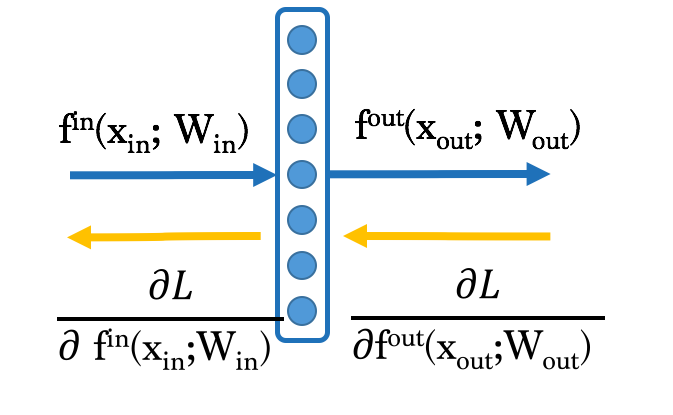
\includegraphics[scale=0.3]{img/bp1}
			
			\begin{itemize}
				\item Gradient wrt parameters 
					$$\frac{\partial L}{\partial W_{out}} = 
						\frac{\partial L}{\partial f^{out}(x_{out}, W_{out})}
						\frac{\partial f^{out}(x_{out}, W_{out})}{W_{out}}  $$
				
				\item Gradient wrt input 
					$$\frac{\partial L}{\partial f^{in}(x_{in}; W_{in})} = 
						\frac{\partial L}{\partial f^{out}(x_{out}, W_{out})}
						\frac{\partial f^{out}(x_{out}, W_{out})}{f^{in}(x_{in}; W_{in})}  $$
			\end{itemize}
		\end{center}
	\end{frame}
	
	\subsection*{Layer Abstarction}
\begin{frame}[fragile]


\begin{itemize}
	\item Affine
	\begin{minted}[fontsize=\small]{python}
class AffineLayer(): 
  def forward(x, params=(w, b)):
    return w.dot(x) + b #compute affine function

  def backward(x, params=(w, b), dout):
    dx = d_x(x, dout) # derivation wrt input 
    dw = d_w(w, dout)  # derivation wrt parametrs  
    db = d_b(b, dout)  # derivation wrt parametrs  
    return (db, dw), dx
	\end{minted}
	
	\item Sigmoid 
	\begin{minted}[fontsize=\small]{python}    
class SigmoidLayer():
  def forward(x, params=()):
    return np.sigm(x) #compute sigmoid function

  def backward(x, () dout):
    dx = dx(x, dout) # derivation wrt input 
    return (), dx
	\end{minted}
\end{itemize}

\end{frame}
	
	\subsection*{How to Train Recurent NN Unwrapping}
	\begin{frame}
		
		RNN

				\begin{center}
					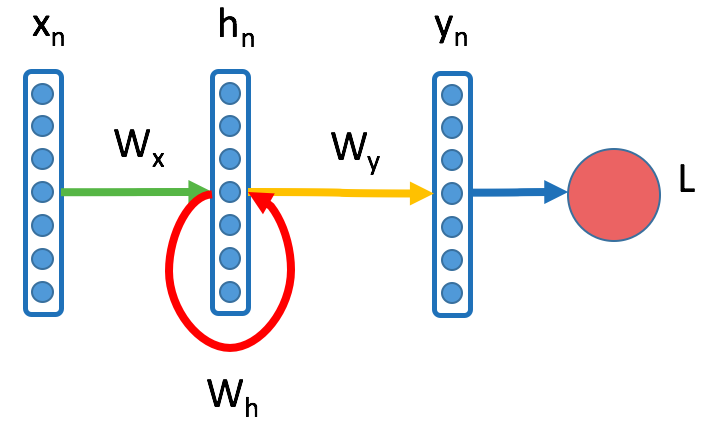
\includegraphics[scale=0.2]{img/rnn}
				\end{center}
				
		Unwrapping RNN

				\begin{center}
					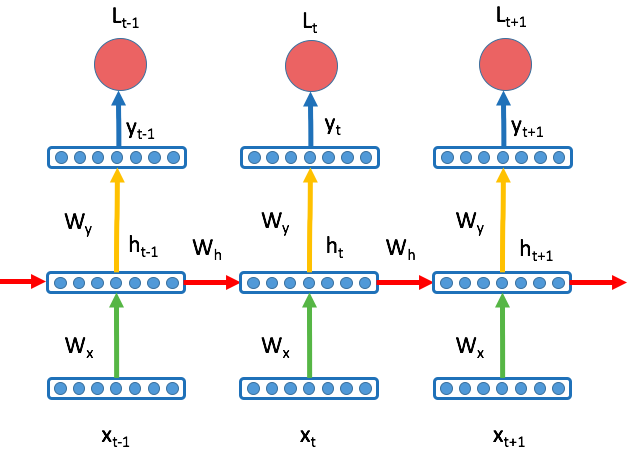
\includegraphics[scale=0.22]{img/rnnw}
				\end{center}		
	\end{frame}
	
	\subsection*{How to Train Recurent NN Math}
	\begin{frame}
		
			\begin{center}
				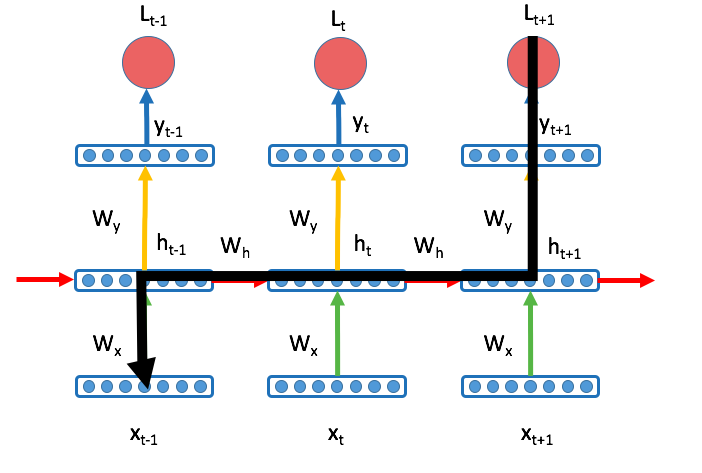
\includegraphics[scale=0.22]{img/rnnw2}
			\end{center}		

			\begin{align*}
				E = \sum_{t=1}^s E_t;~~
				\frac{\partial E}{\partial W_h} = \sum_{t=1}^s \frac{\partial E_t}{\partial W_h};~~ 
				\frac{\partial E_t}{\partial W_h} = 
				\sum_{k=1}^t  \frac{\partial E_t}{\partial y_t} \frac{\partial y_t}{\partial h_t}
				\frac{\partial h_t}{\partial h_k} \frac{\partial h_k}{\partial W_h}\\
				||\frac{\partial h_t}{\partial h_k}|| < const(W)^{t-k}~~~~~~~~~~~~~~~~~~~~~~~~~\\
			\end{align*}
			\vspace{-1cm}
			\begin{tcolorbox}[colback=gray!0, colframe=red!90]
				\centering Gradients \textbf{1)} $const(W) > 1$  Boom~\textbf{2)} $const(W) < 1$  Vanishing 
			\end{tcolorbox}

	\end{frame}
	
	\subsection*{How to Train Recurent NN Vanishing}
	\begin{frame}
		
		\begin{center}
			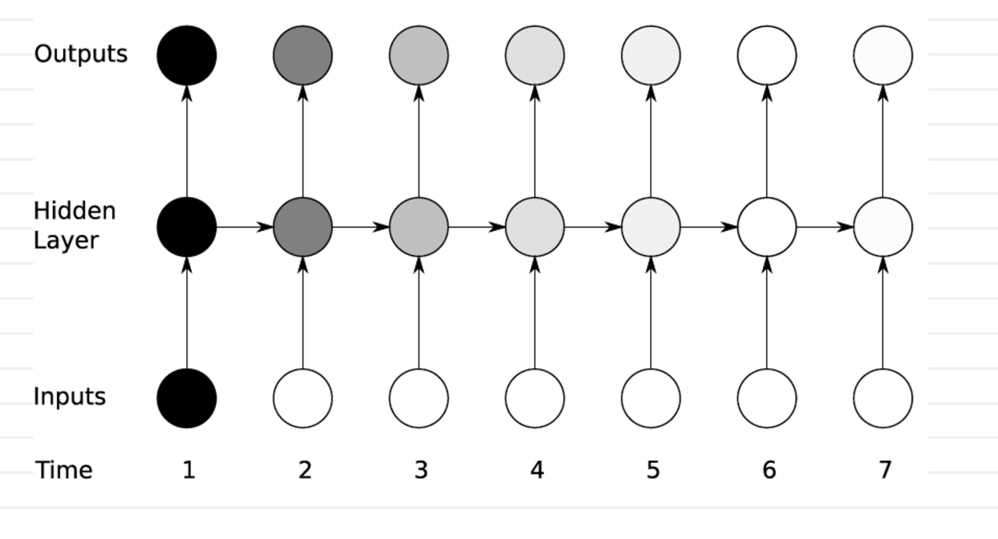
\includegraphics[scale=0.3]{img/van1}
		\end{center}					
	\end{frame}
		

	\section*{Long Short-Term Memory}
	\subsection*{Memory Idea / Interpretation}

	\begin{frame}
			\begin{center}
				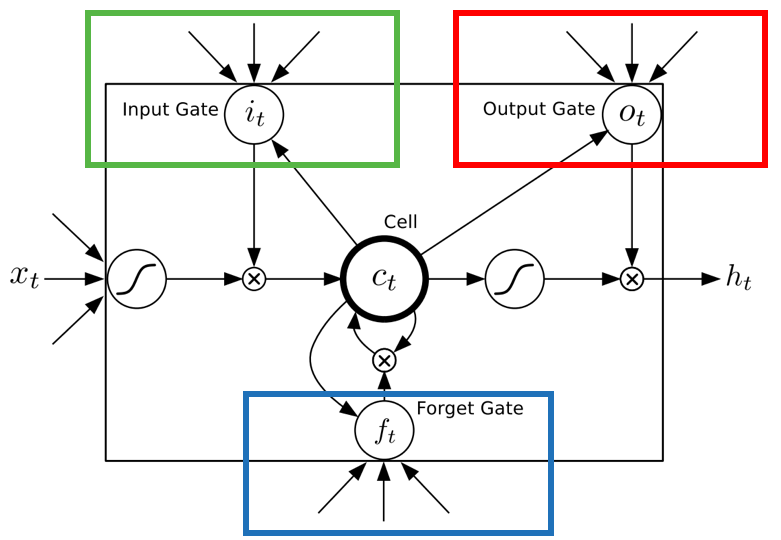
\includegraphics[scale=0.25]{img/lstm2}
			\end{center}
	
			\vspace{-0.6cm}
			\begin{align*}
				y_i = \textcolor{red}{output_i} \odot \sigma(h_t)~~~~~~~~~~~~~~~~~~~\\ 
				h_i = \textcolor{blue}{forget_i} \odot h_{i-1} +  \textcolor{green}{input_i} 
				\odot \sigma(W_x x + W_h h_{t-1})\\
				\textcolor{green}{input_i = \sigma(W^{input}_x x_t + W^{input}_h h_{t-1}+ b^{input}) } \\
				\textcolor{blue}{forget_i =  \sigma(W^{forget}_x x_t + W^{forget}_h h_{t-1}+ b^{forget}) }  \\
				\textcolor{red}{output_i = \sigma(W^{output}_x x_t + W^{output}_h h_{t-1}+ b^{output})} \\
			\end{align*}		
			
	\end{frame}
	
	\subsection*{Cases}
	\begin{frame}
		
		\begin{center}
			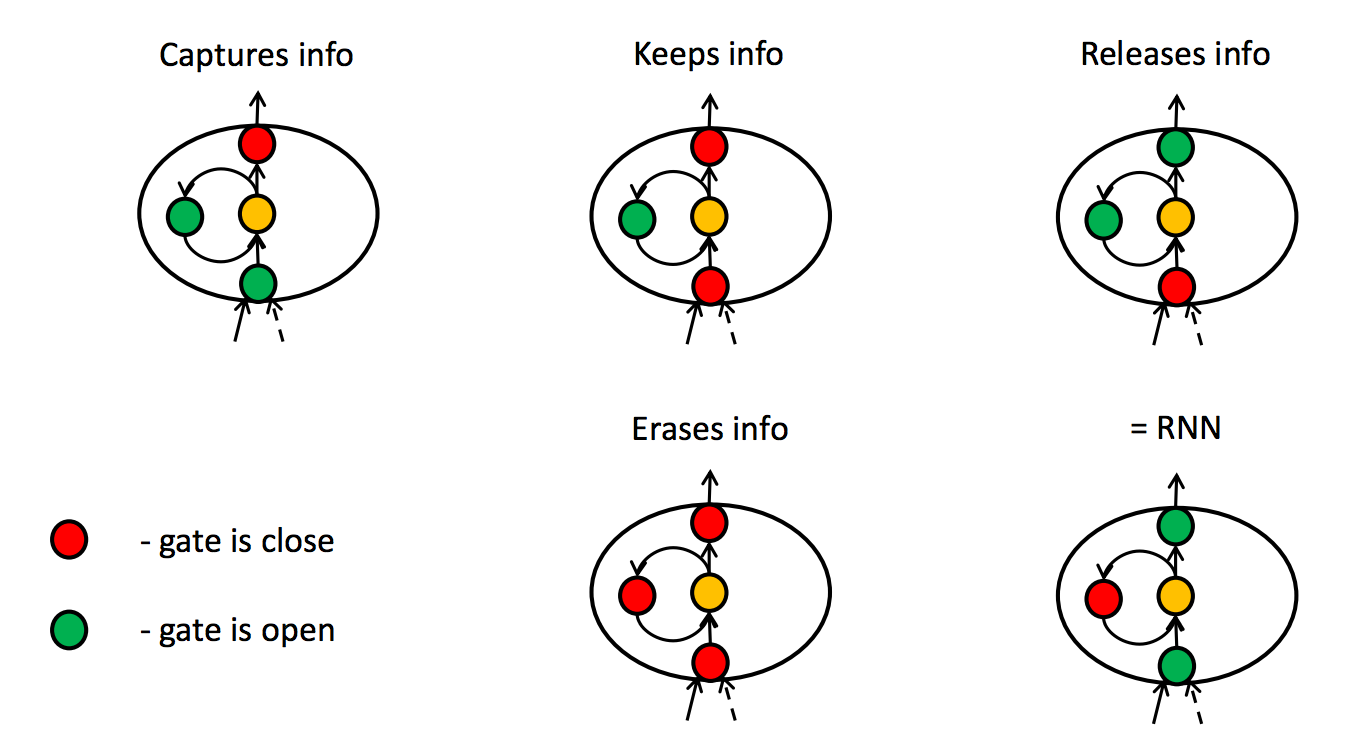
\includegraphics[scale=0.25]{img/cases}
		\end{center}					
	\end{frame}
		
	
	\subsection*{Long Term Depandancies}
	\begin{frame}
		
		\begin{center}
			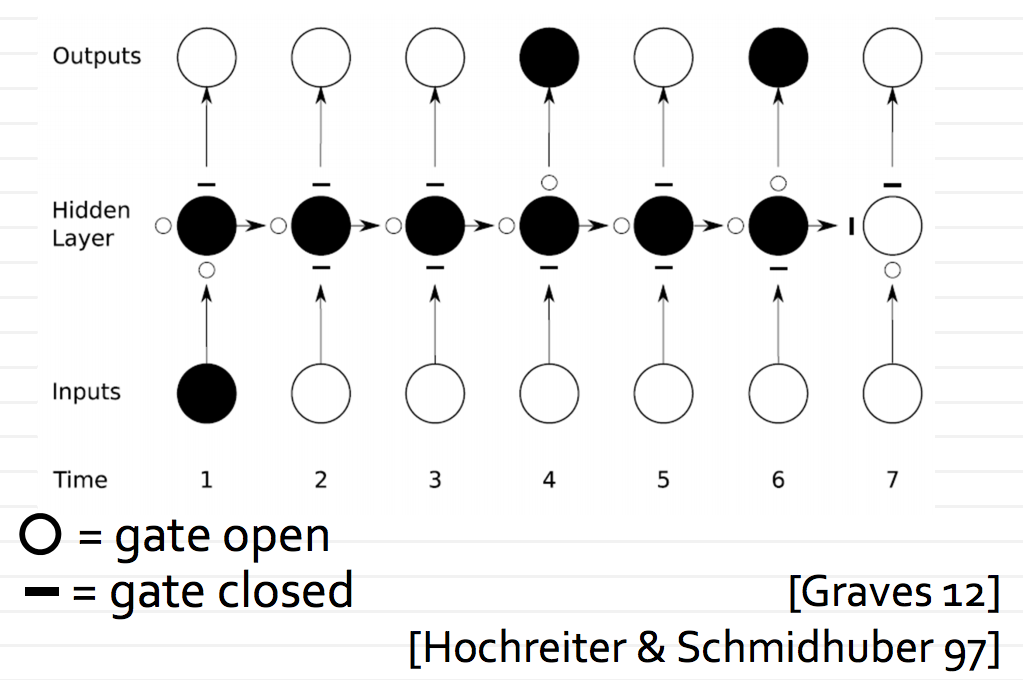
\includegraphics[scale=0.3]{img/van}
		\end{center}					
	\end{frame}
	
	\section*{Examples}
	\subsection{Avito Text Classification}
	\begin{frame}
		\begin{center}
			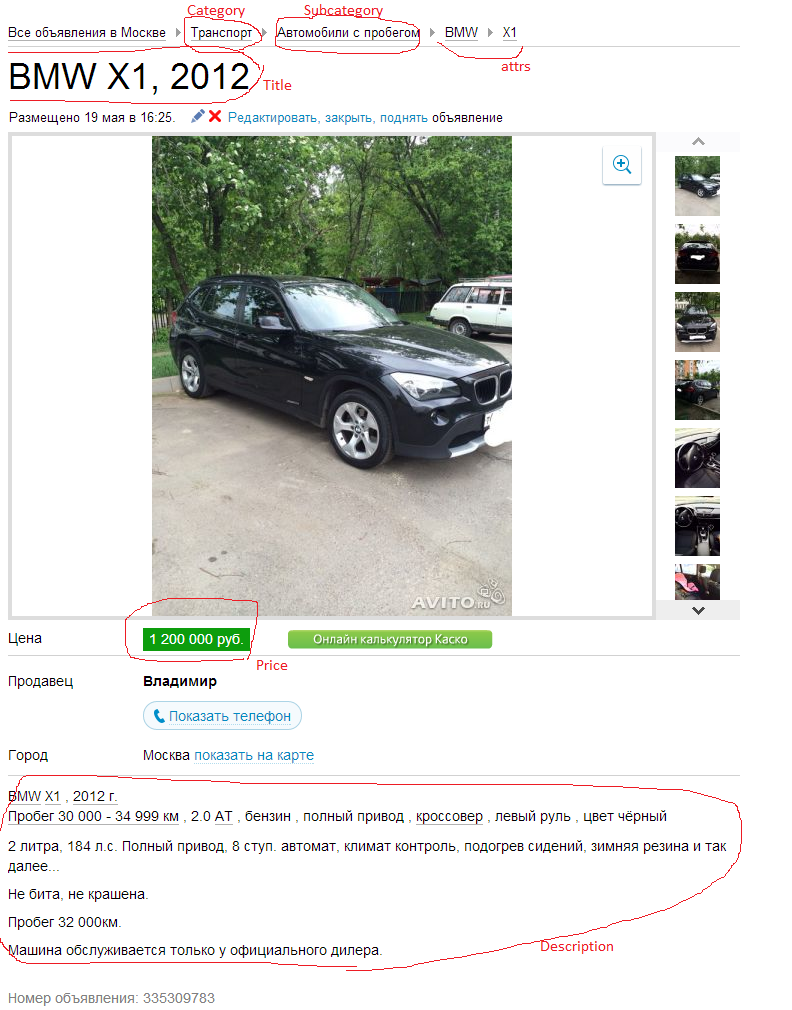
\includegraphics[scale=0.3]{img/avito}
		\end{center}
	\end{frame}
	\subsection{Avito Text Classification}
	\begin{frame}
		\begin{center}
			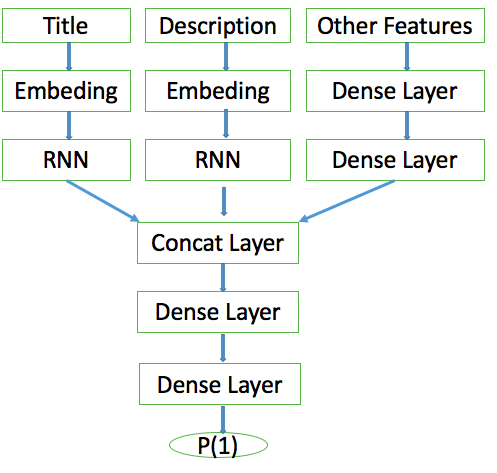
\includegraphics[scale=0.45]{img/clf}
		\end{center}
		\vspace{-0.2cm}
		\begin{enumerate}
			\item Ipython Example
		\end{enumerate}
	\end{frame}
	
	\subsection{Text Generative Models}
	\begin{frame}
		\begin{center}
			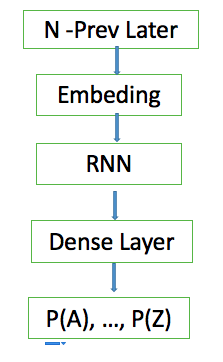
\includegraphics[scale=0.5]{img/gen}
		\end{center}
		\begin{enumerate}
			\item Ipython Example
			\item \href{http://karpathy.github.io/2015/05/21/rnn-effectiveness/}{http://karpathy.github.io/2015/05/21/rnn-effectiveness/}
		\end{enumerate}

	\end{frame}
	
	\subsection{Text-Image Models}
	\begin{frame}
		\begin{center}
			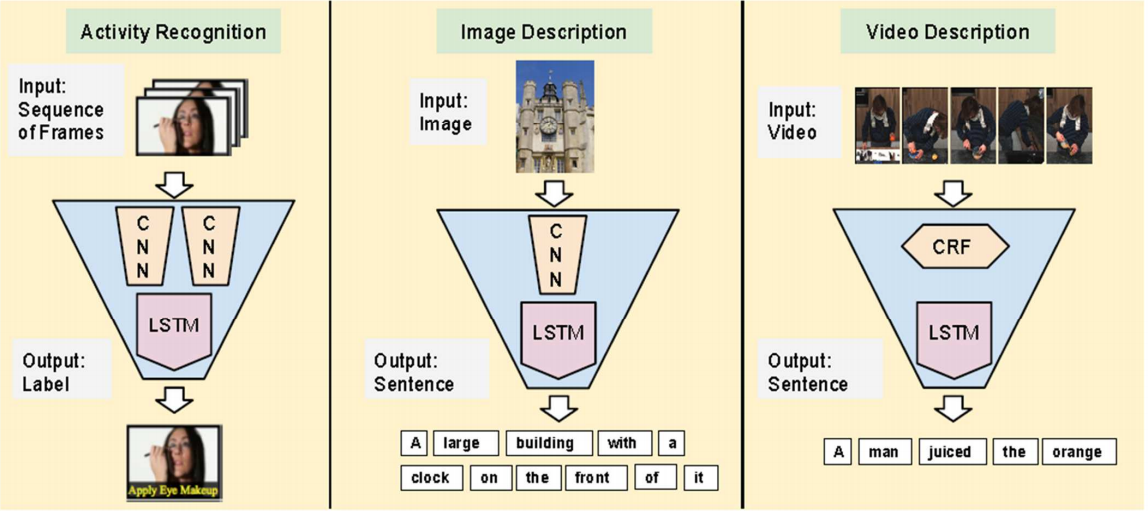
\includegraphics[scale=0.3]{img/im2txt}
		\end{center}
		{\small 
		\begin{enumerate}
			\item \href{http://cs.stanford.edu/people/karpathy/deepimagesent/generationdemo/}
			{http://cs.stanford.edu/people/karpathy/deepimagesent/generationdemo/}
		\end{enumerate}
	}
	\end{frame}

	\subsection{Handwriting Generation}
	\begin{frame}
		\begin{center}
			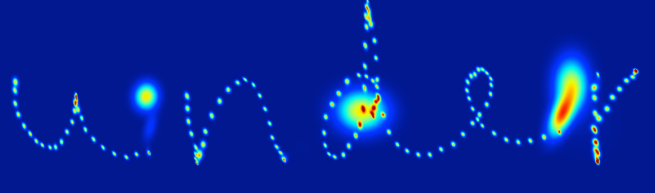
\includegraphics[scale=0.2]{img/hwr1}
			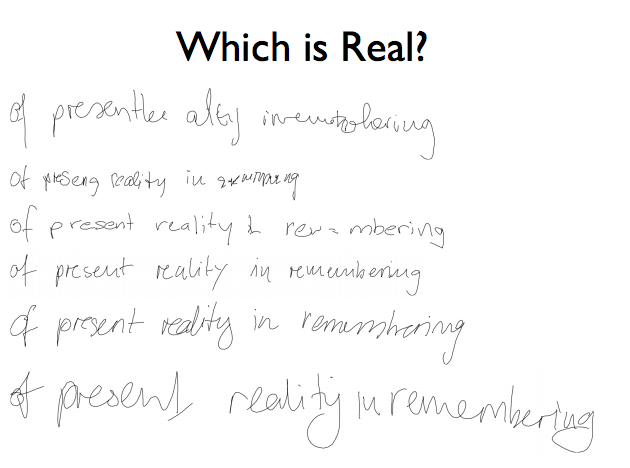
\includegraphics[scale=0.35]{img/hwr2}
		\end{center}
		
		\begin{enumerate}
			\item \href{http://www.cs.toronto.edu/~graves/handwriting.html}{http://www.cs.toronto.edu/~graves/handwriting.html}
			\item \href{http://arxiv.org/abs/1308.0850}{http://arxiv.org/abs/1308.0850}
		\end{enumerate}
	\end{frame}
		
	
	\section*{Resume}
	\begin{frame}
		Advantages
		\begin{itemize}
			\item[+] Learn features automatically 
			\item[+] Complex non-linear Models
			\item[+] Save sequence structure
		\end{itemize}
		
		\vspace{1cm}
		DisAdvantages
		\begin{itemize}
			\item[$-$] Computational hard
			\item[$-$] Hard to optimization (non-convex, ...)
			\item[$-$] Available for Over-fit (how can we solve it?)
		\end{itemize}
		
	\end{frame}
\end{document}

